\section{Methodology}

% We present three key techniques to accelerate diffusion-based language model inference: KV approximation caching, AR-assisted unmasking, and speculative decoding.

% \subsection{KV Approximation Caching}

% \subsubsection{Observation: Attention Decay}

% In non-causal attention, contributions from future tokens to past positions decay rapidly. We exploit this by freezing early-layer key/value states during denoising.

% \subsubsection{Implementation}

% We define an effective cache truncation threshold $\epsilon$, below which the attention contribution is negligible:
% \[
% \text{Mask}(i, j) = \mathbb{1}[ \alpha_{ij} > \epsilon ]
% \]

% \subsection{AR-Assisted Unmasking}

% We use a lightweight AR model to suggest the next token(s), guiding the denoising process.

% \subsection{Speculative Decoding with Verifier}

% A strong AR verifier accepts or rejects unmasked tokens proposed by the diffusion model. Rejected spans are re-noised and regenerated.


% \subsection{Preliminary of Diffusion Language Model}

% Given the partially masked token sequence $\mathbf{x}_t$ at step $t$, assume the diffusion language model $f_\theta$ will complete the sequence with $T$ denoising steps. 
% \zhanqiu{TODO: Mention specifics for diffusion language model: unmasking}


% Diffusion language models (DLMs) generate sequences by progressively denoising an initially masked token sequence over $T$ iterative steps. At each timestep $t$, the model $f_\theta$ predicts token distributions given the current partially masked sequence $\vec{x}_t$. While DLMs enable parallel token generation and bidirectional attention, their inference remains inefficient due to repeated full-sequence forward passes. We propose two complementary techniques---KV approximation caching \zhanqiu{TODO: might want to rename this} and AR-guided unmasking---to improve inference efficiency and scalability without loss in quality.

\subsection{Preliminary of Diffusion Language Model}\label{sec:preliminary}

Diffusion language models (DLMs) generate sequences by iteratively unmasking an initially masked token sequence over \(T\) denoising steps. Mathematically, let \(\mathbf{x}_T\in\mathbb{N}^L\) be the fully masked input (all positions set to $\texttt{[MASK]}$), where the still masked position $M_t$ is represented as:
\begin{equation}
M_t = \bigl\{\,i : x_t[i] = \texttt{[MASK]}\bigr\}
\end{equation}
At each iteration \(t=T,\dots,1\), the model \(f_\theta\) produces logits
\begin{equation}
z_t = f_\theta(\mathbf{x}_t)\quad\text{for }i\in M_t,
\end{equation}

from which a subset \(U_t\subseteq M_t\) of positions is selected (e.g.\ by confidence scoring) and filled via: 
\begin{equation}
\mathbf{x}_{t-1}[i]
= \arg\max_{v\in\mathcal V}\bigl[\mathrm{Softmax}(z_t[i])\bigr],\quad i\in U_t,
\end{equation}

yielding the next mask set \(M_{t-1}=M_t\setminus U_t\).  By repeating this denoising and unmasking process until \(M_0=\emptyset\), the model produces the final fully unmasked sequence \(\mathbf{x}_0\).

% While this parallel unmasking with bidirectional attention allows all positions to be updated simultaneously, it incurs an additional factor of \(O(L)\) cost per step from recomputing full‐sequence forward passes. In addition, quality drops significantly as the size of the unmasked set $U_t$ increases. In this work, we address this inefficiency with two complementary training-free techniques, KV approximation caching \zhanqiu{Rename} and AR-guided unmasking, which accelerate inference without compromising quality.  



\begin{table}[h!]
\centering
\renewcommand{\arraystretch}{1.1}
\resizebox{0.95\linewidth}{!}{\begin{tabular}{llcc}
\toprule
\textbf{Module} & \textbf{Operation} & \textbf{Auto-Regressive LM (decode)} & \textbf{Diffusion LM (length $L$)} \\
\midrule
\multirow{4}{*}{MHA} 
& $W_Q$, $W_K$, $W_V$ projections & $\mathcal{O}(d^2)$ & $\mathcal{O}(Ld^2)$ \\
& Query $\times$ Key ($QK^\top$) & $\mathcal{O}(l^2 d / h)$ & $\mathcal{O}(L^2 d / h)$ \\
% & Softmax + scaling              & $\mathcal{O}(l^2)$        & $\mathcal{O}(L^2)$ \\
& Attention Score $\times$ Value           & $\mathcal{O}(l d / h)$ & $\mathcal{O}(L^2 d / h)$ \\
& Output projection ($W_{\text{out}}$) & $\mathcal{O}(d^2)$ & $\mathcal{O}(L d^2)$ \\
\midrule
\multirow{2}{*}{FFN}
& $W_1$ projection               & $\mathcal{O}(d \dot d_{\text{ff}})$ & $\mathcal{O}(L d d_{\text{ff}})$ \\
& $W_2$ projection               & $\mathcal{O}(d d_{\text{ff}})$ & $\mathcal{O}(L d d_{\text{ff}})$ \\
\bottomrule
\end{tabular}}
\vspace{1.0em}
\caption{Compute complexity of Transformer modules: AR decodes a prefix of length \(l\) per token vs. DLM processes full length \(L\) each denoising step.}
\label{tab:transformer-complexity}
\end{table}

\subsubsection{Bottleneck of Diffusion Language Model Inference}

While diffusion models allow parallelized generation of tokens, this comes at the expense of extra computation overhead per forward pass. 
Given the input $x_T$ with sequence length $L$, each forward pass of the diffusion model $f_\theta$ requires full-sized computation~(both current and past tokens) throughout the multi-head attention~(MHA) block and feed-forward network~(FFN) of the transformer model. 
Unlike the autoregressive model where the past tokens are cached for the new token generation, diffusion model produces output without the consideration of causality. 
As shown in Table~\ref{tab:transformer-complexity}, DLM models introduce an additional computational complexity of $O(L)$ at each module of a transformer-based model architecture. 
As a result, the latency overhead introduced by the DLM architecture is massive compared to the Auto-Regressive Model, as shown in the comparison in Section~\ref{sec:res}. 
Based on the theoretical analysis above, the first challenge of the diffusion model is: 

\textbf{Challenge}\circled{1}: \textit{How to alleviate the latency and computation overhead caused by the liability of full sized cache computation of DLM?}


% it incur an additional factor of \(O(L)\) cost per step from recomputing full‐sequence forward passes. 

% In addition, quality drops significantly as the size of the unmasked set $U_t$ increases. In this work, we address this inefficiency with two complementary training-free techniques, KV approximation caching \zhanqiu{Rename} and AR-guided unmasking, which accelerate inference without compromising quality.  

% Let L denote the full sequence length, which is equal to the sum of input token length and context window length for generation tasks. Each $f_\theta$ is a full forward pass of a transformer decoder with input sequence length of L, which includes multi-head attention (MHA) and feedforward (FFN) layers, applied to the entire sequence at every timestep.

% Table~\ref{tab:transformer-complexity} highlights a key contrast in forward pass efficiency between autoregressive models and diffusion models. Autoregressive decoding operates on a growing prefix of length $l$, while diffusion models operate on the full sequence of length $L$ at each denoising step. All linear projections in DLM scale with $L$ compared to the constant size in ARM. 

% Most linear projections in ARM involve matrix-vector multiplication (e.g., $\mathbb{R}^{d \times d} \cdot \mathbb{R}^{d \times 1}$), while DLM requires matrix-matrix multiplication ($\mathbb{R}^{d \times d} \cdot \mathbb{R}^{d \times L}$), leading to significantly higher computational cost.


\subsubsection{Token Incoherence in Parallel Generation}\label{sec:incor}

% Another fundamental challenge in diffusion-based language models is what we refer to as the 
As introduced in Section~\ref{sec:preliminary}, DLM irregularly unmasks output token positions throughout diffusion process. As a result, simultaneously unmasking token positions without semantical correlation leads to insufficient semantical consistency, which can further degrades the model performance. 
While the desire of preserving the parallel diffusion persists. Figure~\ref{fig:bars} shows accuracy degradation with decreasing denoising steps for three diffusion sampling methods: MaskGIT~\cite{chang2022maskgitmaskedgenerativeimage}, entropy-based, and Top-K Margin~\cite{kim2025trainworstplanbest_topkmargin}.  The challenge arises as follows: 

\textbf{Challenge}\circled{2} \textit{How to enhance the semantic correlation of the diffusion process \textbf{ without} introducing additional training and fine-tuning effort? }

% As presented recent studies of reinforcement learning, understand the semantical logic and causality of given context is critical for high performance reasoning. 
Motivated by the aforementioned challenges, we propose a novel approach which directly accelerates the diffusion model in a simple, effective, and systematic manner. 
% \textit{When multiple masked positions are predicted and unmasked simultaneously without coordination, each prediction is made independently without conditioning on each other. This can lead to unmasked tokens violating semantic or grammatical consistency, leading to quality degradation. }

% At each denoising step, the model predicts all masked tokens simultaneously. While this enables high parallelism, it often leads to inconsistent or grammatically invalid token combinations—e.g., ``an cat'', ``a elephant'', ``two is'', or duplicated entities—because the model lacks an explicit mechanism for enforcing consistency across tokens predicted in the same step. 

% For example, unmasking multiple tokens in one denoising step might resulting in incorrect token combindations (e.g., ``an cat'', ``a elephant'', ``two is''), or duplicated entities, because the model lacks an explicit mechanism for enforcing consistency across tokens predicted in the same step. 

% This issue arises because predictions at each position are made in parallel, conditioned on a partially masked context, without coordinated control over the semantics of jointly predicted tokens. We refer to such mismatched outputs as token-incoherent generations.

% Recent approaches such as MaskGIT~\cite{} and \zhanqiu{TODO: cite more} attempt to mitigate this using heuristic confidence scores or sampling rules based on predicted token probabilities. 

% However, these heuristics do not model token interactions explicitly, and often degrade generation quality when unmasking multiple tokens per step. As a result, diffusion models are forced to unmask conservatively, increasing the number of denoising steps and reducing inference efficiency.


% However, these heuristics do not model token interactions explicitly, and often degrade generation quality with decreasing denoising steps. Figure \ref{fig:pareto} \zhanqiu{Replace table, add description} shows the accuracy degredation with the average number of tokens generated at each step (generated tokens / denoising steps).



% To address this limitation and fully exploit the parallelism of diffusion-based generation, we propose a principled solution: \textit{guided diffusion}. Our method leverages a lightweight pre-trained autoregressive model (ARM) to provide alignment supervision during inference: masked tokens predicted by the diffusion model are only unmasked when they are consistent with the ARM’s sequential predictions. This cross-model agreement serves as a lightweight coherence prior, enabling the model to safely unmask multiple tokens in parallel, without requiring any additional training or fine-tuning.

% In contrast to prior heuristic-based methods (e.g., confidence thresholds or top-$k$ logits), which often suffer from severe quality degradation when unmasking more than a few tokens per step, guided diffusion maintains fluency and correctness even under aggressive unmasking. This substantially reduces the number of denoising steps, often by a factor of 5× or more, without compromising output quality.

% We provide detailed comparisons in Section~\ref{sec:experiments}, \zhanqiu{TODO} showing that guided diffusion achieves significantly faster inference and stronger generation quality compared to baseline sampling strategies.



% DLM predicts the entire sequence for the next timestep. SOTA approaches use heuristics such as maskgit~\cite{} \zhanqiu{check qwen paper for sampling strategy} that compute a confidence score based on predicted logits for masked tokens, and greedily unmask tokens with high confidence scores. 

% However, tokens generated in parallel might be interdependent, unmasking interdependent tokens in the timestep will result in false token combinations being predicted. Heuristic sampling strategies do not have a mechanism that prevents this. Therefore, unmasking multiple tokens in one step results in a significant quality drop in generated sequences. 

% \zhanqiu{Add data here}

% This prevents us from exploiting the parallelized generation of diffusion language models without drop in quality. To solve this problem, we proposes guided diffusion techniques that leverage a pre-trained lightweight autoregressive model to guide unmasking strategies, achieving aggressive unmasking without quality drop. 

% \begin{figure}[t]
\begin{figure}[t]
  \centering
  \begin{subfigure}[t]{0.5\textwidth}
    \centering
    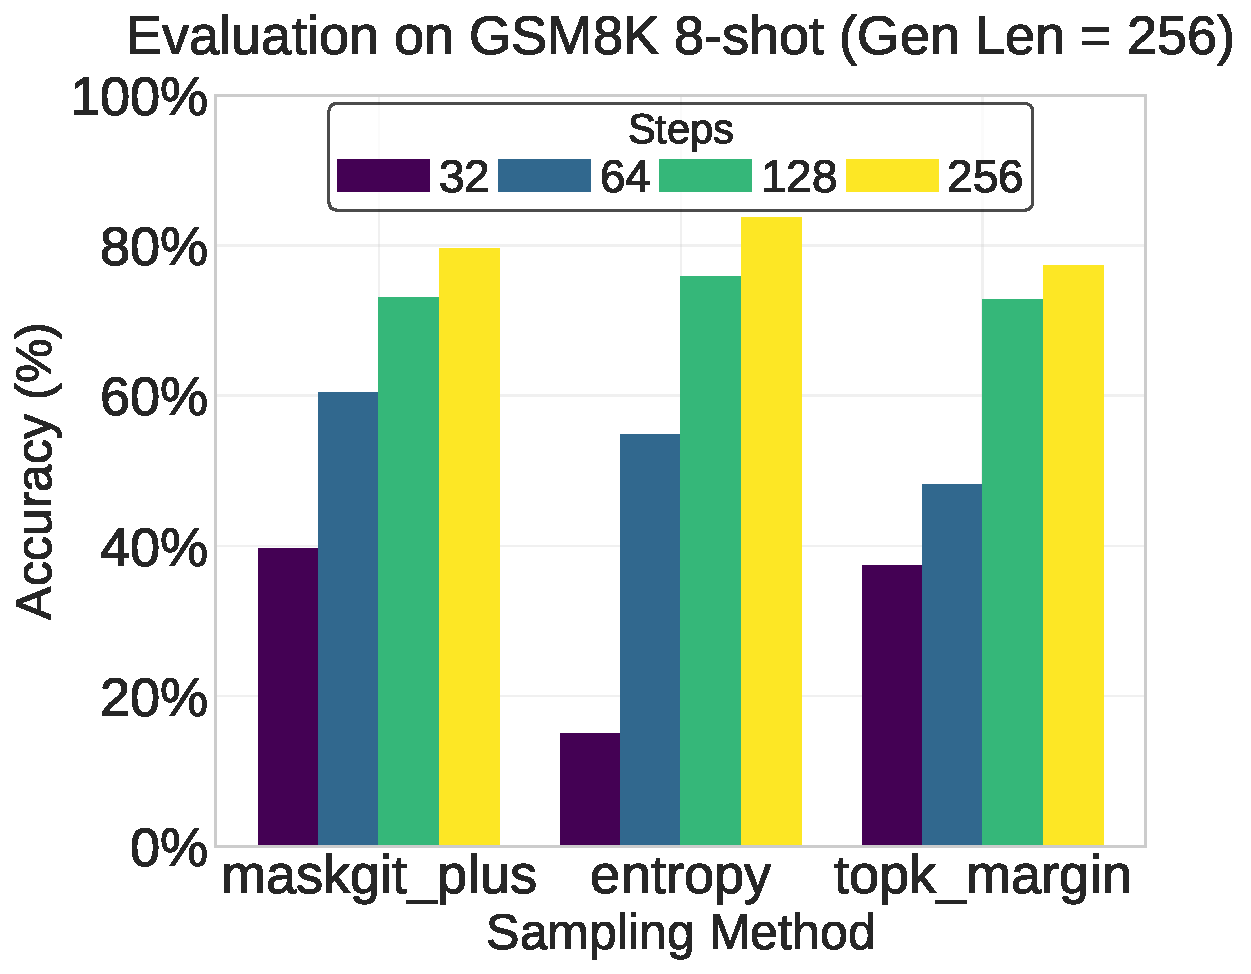
\includegraphics[width=\linewidth]{sections/method/figures/algorithm_comparison.pdf}
    \caption{
      \textbf{Quality degradation from aggressive unmasking.}
      Heuristic methods suffer from significant accuracy loss with decreasing denoising steps.
    }
    \label{fig:bars}
  \end{subfigure}
  \hfill
  \begin{subfigure}[t]{0.48\textwidth}
    \centering
    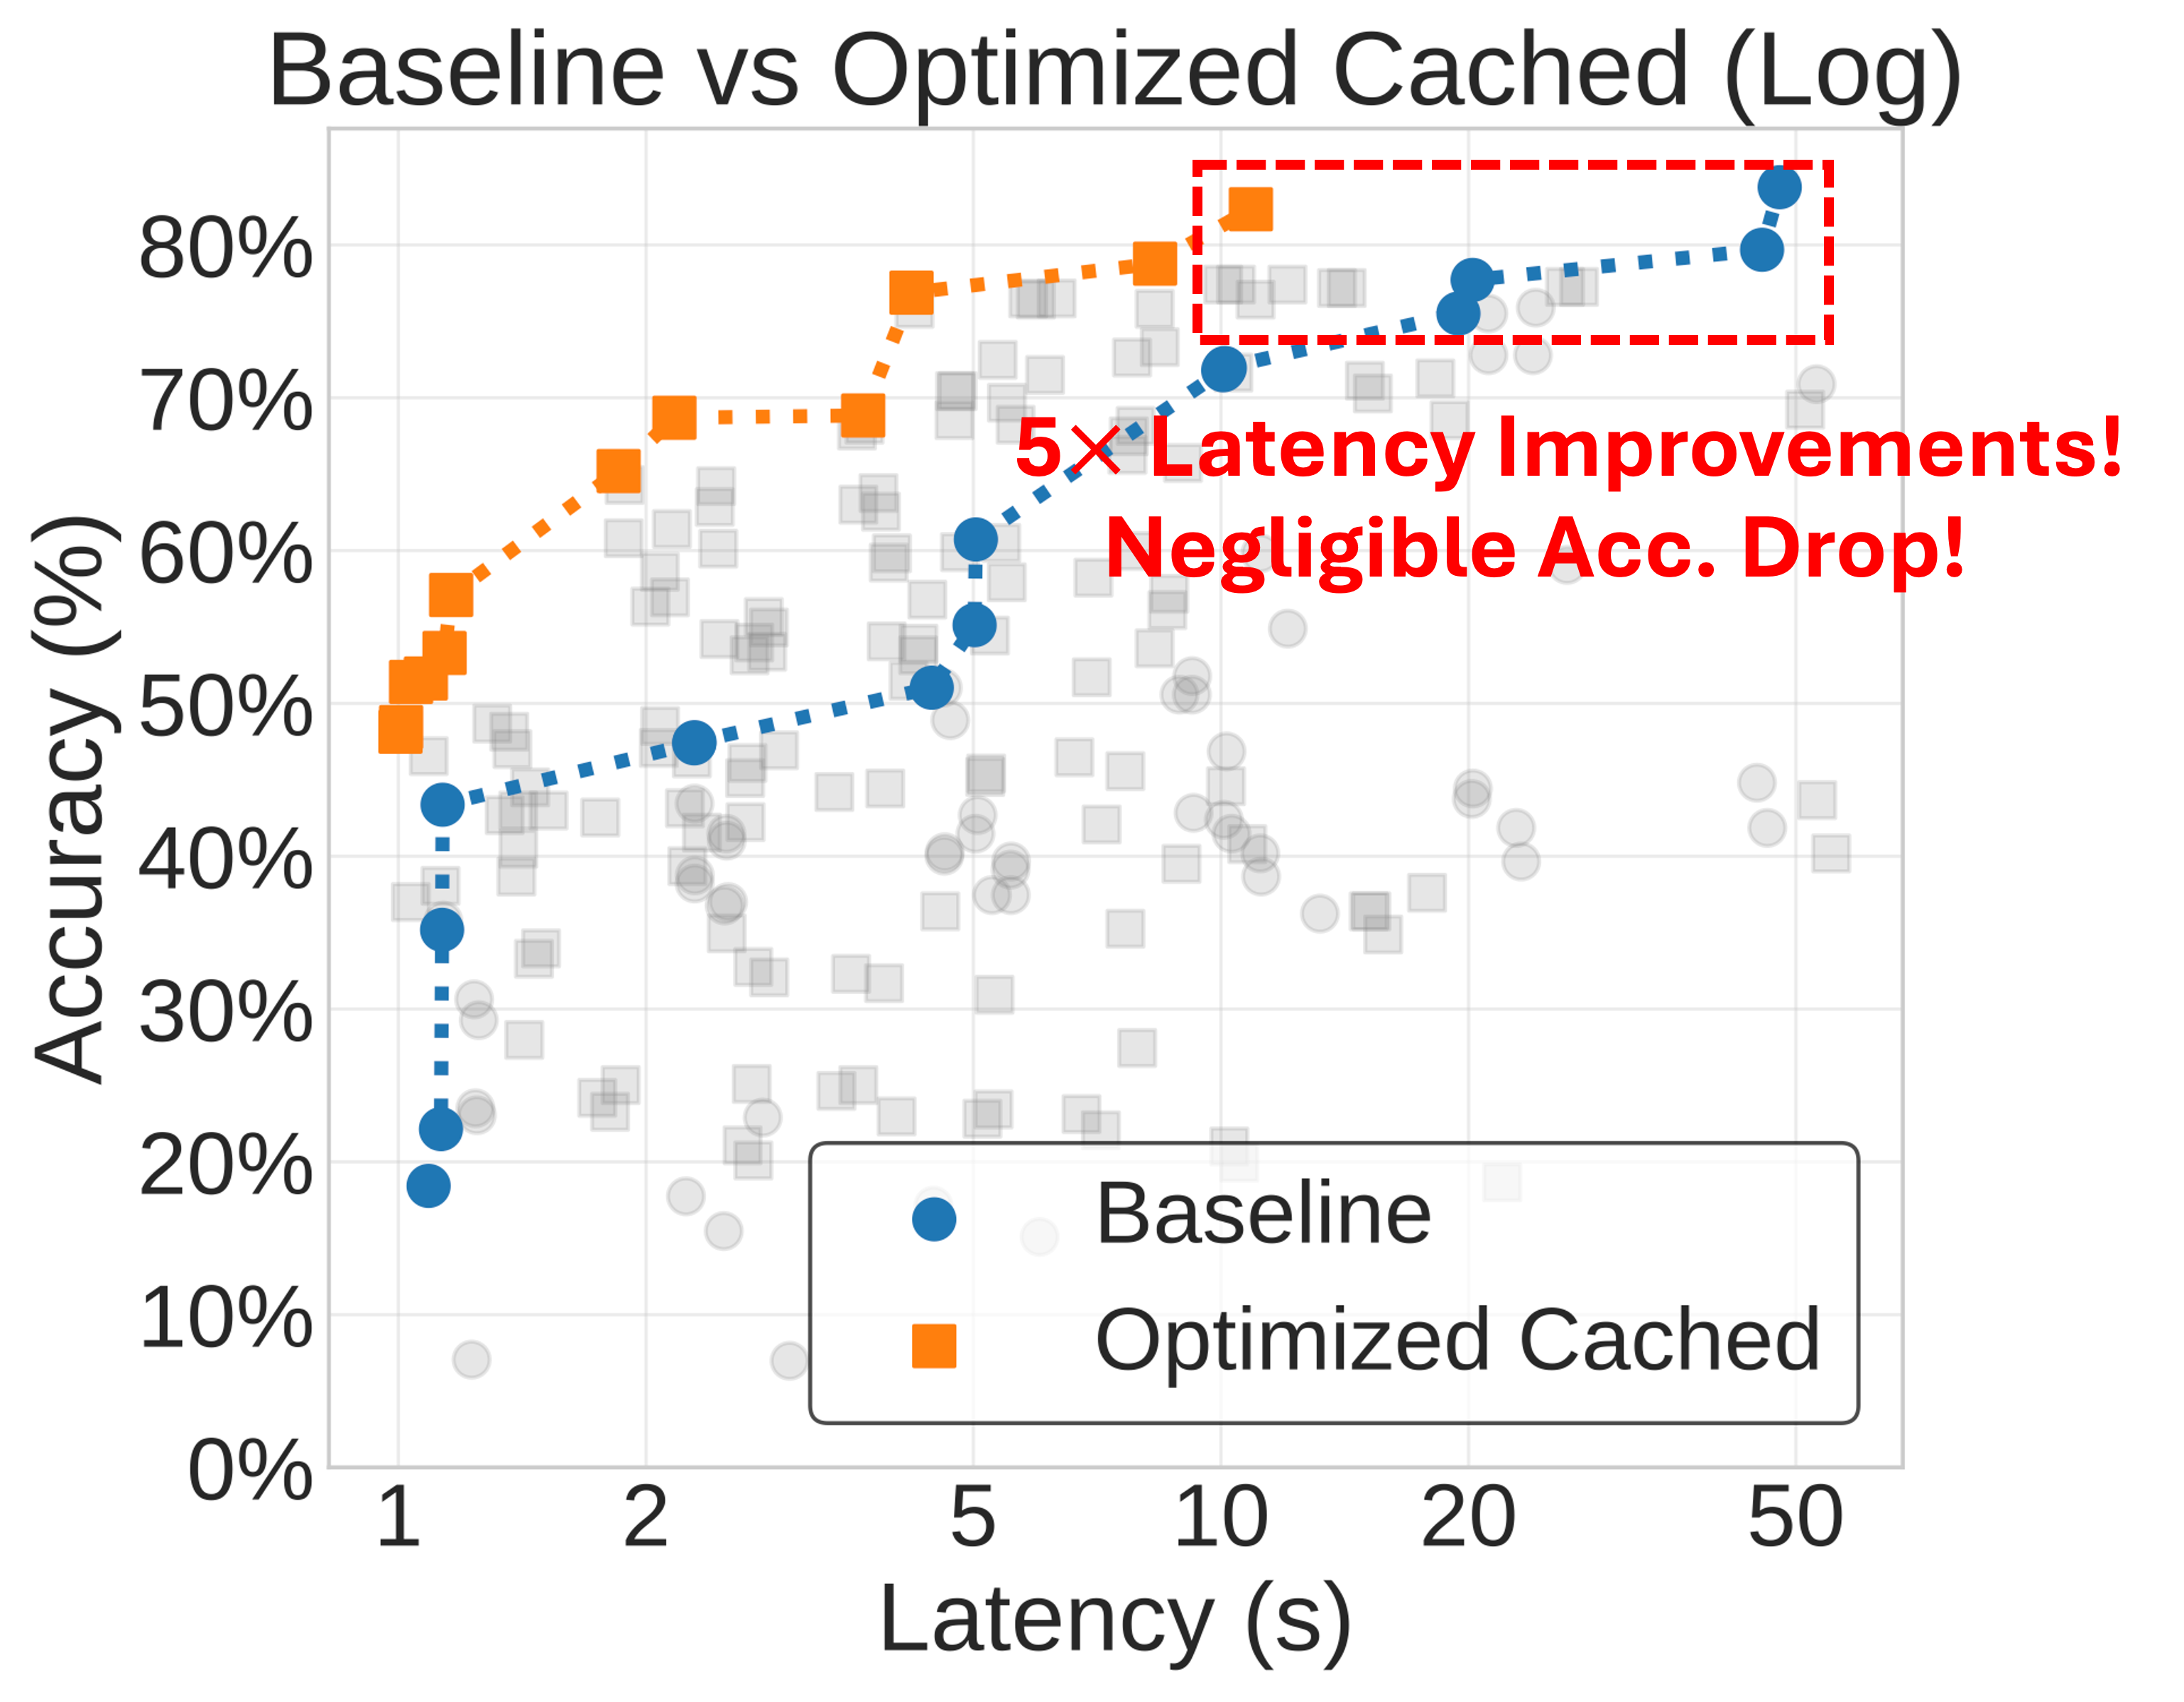
\includegraphics[width=\linewidth]{sections/method/figures/overlay_baseline_vs_optimized_cached_log_latency_v2.png}
    \caption{
      \textbf{Latency–accuracy tradeoff.}
      Pareto front comparing the standard autoregressive baseline with our KV‐cache optimized method, highlighting substantial latency reductions at equivalent accuracy levels.
    }
    \label{fig:kvcache}
  \end{subfigure}
  \caption{
    {\bf (a)} Quality degradation under aggressive unmasking. 
    {\bf (b)} Pareto front of accuracy vs.\ latency (log‐scale) for baseline and optimized cached methods.
  }
  \label{fig:combined_pareto}
\end{figure}


\subsection{Proposed Method}
% This section presents two methods that directly accelerate the SoTA diffusion model off-the-shelf. 
% To address both the quadratic compute growth and the token incoherence inherent to naïve diffusion inference, we introduce two complementary, training‐free components.  

% \textbf{FreeCache.} 
% We exploits the observation that once a contiguous block of tokens has been fully unmasked, its influence on earlier blocks remains effectively fixed; by caching and reusing each block’s key/value projections, we reduce the per‐step attention cost from \(O(L)\) to \(O(B)\), where \(B\) is a user‐defined block size.  

% \emph{Guided diffusion} leverages a lightweight pre-trained autoregressive model to guide parallel unmasking: at each denoising step, we unmask tokens where the DLM and ARM agree. This enforces coherence under aggressive unmasking and reduces the number of denoising steps by over \(5\times\) without any drop in generation quality.  





% Under the context of natural language processing, the correlation between different tokens~(words) follows the order of logic. 
% Autoregressive language models~(ARM) use causal masks to enforce causality throughout the inference process. 
% Interestingly, our observation shows that the context correlation persists even within the non-causal, fully bidirectional attention of the well-trained diffusion language models. 
% During the steps of DLMs, the contribution of masked tokens to earlier unmasked ``clean'' tokens diminishes rapidly over denoising steps. This insight enables us to exploit caching the Key and Value states of the ``clean'' tokens and reuse them across future steps without noticeable quality degradation, namely, the \texttt{FreeCache}.


% \textit{Initial clean token caching}: 
% Naturally, the input sequence $x_T$ of the diffusion model can be split into prompt tokens $x_P$ and masked dirty tokens $x_G$. 
% Correspondingly, the input query, and key states tensors of each attention block includes the pair of $[Q_P, Q_G]$, $[K_P, K_G]$, respectively. 
% \begin{align}
% Q &= \begin{bmatrix}Q_P \\[4pt] Q_G\end{bmatrix}, 
% \quad
% K = \begin{bmatrix}K_P \\[4pt] K_G\end{bmatrix}, 
% \end{align}
% Therefore, the computation of attention can be represented as the block-wise format as follow: 
% \begin{align}\label{eq:block_diff}
% Q\,K^T
% &= \begin{bmatrix}
% Q_P\,K_P^T & Q_P\,K_G^T \\[6pt]
% Q_G\,K_P^T & Q_G\,K_G^T
% \end{bmatrix},
% \end{align}

% We characterize the impact of each block of $Q\,K^T$ throughout the entire diffusion process~(step 1 to $T$) based on the SoTA Dream-7B-Instruct~\cite{dream2025} model. 
% As shown in Figure~\ref{fig:freecache_rationale},$[Q_P\,K_P^T]_t$ is highly correlated~(within 0.9 and 1.0) with the initial state at each step of the diffusion process, in comparison to other partial attention blocks. 
% Such observation motivates us to exploit the plausibility of caching the Key States that correspond to the prompt tokens of input. In other words, the cached $K_P$ approximates the $Q_P\,K_P^T$. 

% We adopt a \textbf{block-wise} generation scheme. We pre-allocate a K/V cache for the full context length (prompt + generation) and populate it in one initial forward pass. The prompt's K/V is then frozen. Generation proceeds block-by-block. The current block's Query attends to the entire, full-context K/V cache. This cache is dynamically updated by recomputing the current block's K/V, which is then frozen once fully unmasked. For each active block, we run denoising while letting its Queries attend to the full K/V cache (frozen prompt + previously finalized blocks + a cached initialization for future masked tokens). Once the block becomes fully unmasked and stable, we compute its K/V once, freeze them into the global cache, and advance to the next block. This avoids recomputing attention over the entire sequence of length $L$ at every step: only the Queries for the current block of size $B$ are recomputed, while K/V elsewhere are reused. Consequently, per-step compute scales with $B$ rather than $L$. According to Eq~\ref{eq:block_diff}, this reuse preserves the $Q_P\,K_P^T$ interaction and approximates $Q_P\,K_G^T$, yielding substantial speedups with minimal quality impact. 

\subsubsection{FreeCache: Reducing Window Caching for DLM Inference}
\label{sec:freecache}
A key insight for optimizing the generation process in Diffusion Language Models is that the Key and Value (KV) projections for the clean portions of a sequence exhibit high temporal stability. Although these projections are not strictly unchanging, they quickly converge and undergo only negligible changes once a token is finalized.

Figure 2 shows a heatmap that validates the rationale behind our FreeCache method: the temporal stability of KV projections for clean tokens. The y-axis represents the denoising step and the x-axis represents the token position, while the color intensity shows the similarity of a token's value projection to its previous step. Bright yellow indicates high similarity (minimal change), while dark blue signifies a large difference. We observed that the prompt region remains stable across denoising steps, and the generation region illustrates how tokens transition from a low-similarity, unstable state (dark blue) to a high-similarity, stable state (bright yellow) as they become unmasked.

% \begin{figure}[t!]
\begin{figure}[H]
    \centering
    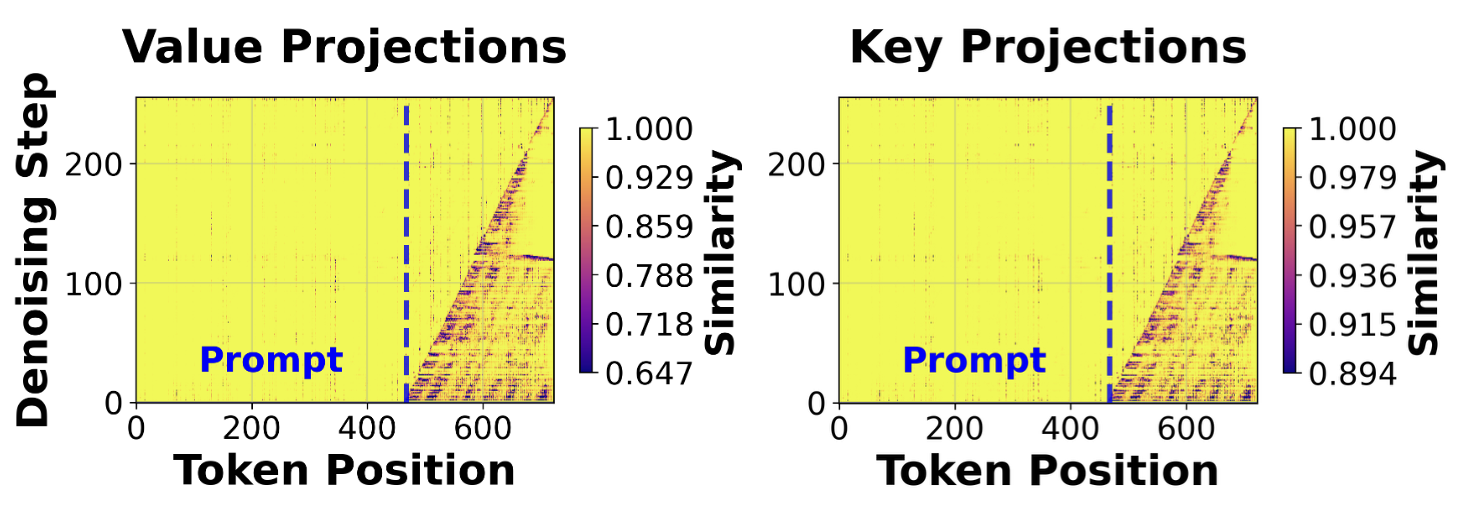
\includegraphics[width=1\linewidth]{sections/method/figures/kv_projections.png}
    \caption{Rationale behind the proposed FreeCache: The variation of K and V projections of clean tokens is small throughout the subsequent diffusion steps. }
    \label{fig:freecache_rationale}
\end{figure}




To exploit this, we propose \texttt{FreeCache}, a reducing window caching strategy where the set of actively computed tokens dynamically shrinks as blocks of the sequence are finalized. The algorithm proceeds as follows: \textbf{Initialization and Partitioning:} The post-prompt generation sequence is partitioned into fixed-size blocks ($B_1, ..., B_N$), and an initial forward pass computes and saves the full KV projections for the entire sequence (prompt + all blocks). \textbf{Windowed Re-computation:} To generate a block $B_i$, the \textbf{active computation window} is defined as $B_i$ and all subsequent blocks ($B_{i+1}, ..., B_N$). KV projections are recomputed only for tokens within this window until $B_i$ is fully unmasked, using all prior frozen blocks and the prompt as context. \textbf{Progressive Caching:} Upon completion of a block $B_i$, its KV projections are \textbf{frozen} for subsequent steps. The active window then shrinks to exclude this block for all subsequent generation steps.

This cascaded approach means that the computational cost per step progressively decreases throughout the inference process, as the active window shrinks with each completed block. This effectively reduces the overall computational overhead, especially for long sequences.


We quantify the performance degradation caused by the \texttt{FreeCache} in Figure~\ref{fig:kvcache} with the 8-shot GSM8K dataset. 
The reducing window caching strategy introduces up to 5$\times$ speedup compared to the vanilla Dream-7B, while preserving the minimal accuracy drop. As shown in Table~\ref{tab:freecache_results}, the proposed FreeCache achieves up to 4.42$\times$ speedup for Dream-7B-Instruct and 6.32$\times$ for LLaDA-8B-Instruct, while maintaining accuracy close to the baseline. We solidify the performance of the proposed method in Section~\ref{sec:res} with further analysis with benchmarks across different domains.





% Although the speedup is achieved with the proposed caching strategy, we further propose a novel method to completely recover the accuracy degradation while exploit the acceleration even further. 
% \textit{Blockwise semi-autoregressive diffusion}: 
% For the remaining masked positions we split them into contiguous blocks of size 
% B. At each step, we only pass the current block to the model. We iteratively repeat the denoising process on the current block until the current block is fully unmasked, and then cache the projected KV corresponding to this block and move on to the next block. This keeps generation within local block diffusive, \zhanqiu{correct word?}, while introducing blockwise auto-regressiveness. This semi-autoregressive diffusion approach reduce input length in subsequent steps from $L$ to $B$, where $B$ is a user-defined value smaller or equal to the context length. 

% \textit{Early exit:} On top of block-wise caching, we implemented an early stopping mechanism that exits generation when an end-of-text token is unmasked and all tokens before the eos are unmasked. 


% In practice, FreeCache \zhanqiu{Rename} yields 5× \zhanqiu{Fill with more data} reduction in generation latency compared with the baseline Dream 7B without measurable degradation in accuracy. It significantly reduces the computation for long sequence generation. Detailed results are presented in Section~\ref{sec: experiments}.

% The semi-autoregressive generation and early stopping enhances each other: we observe that with fully diffusion language model, when the provision context length is longer than the actual generated token, it tends to unmask later tokens as EOS tokens before unmasking actually meaningful tokens (this is especially obvious in tasks like Hellaswag)

% Algorithm:
% 1. In the first denoising step, we pass in the full sequence. We cache the projected keys and values of the cleaning tokens (i.e., the prompt tokens in generation tasks)

% 2. For later steps, splitting the target masked sequence into several blocks and generating them from left right. Caching the each block when they become fully unmasked. This keeps generation within local ... diffusive while introducing blockwise auto-regressiveness. This semi-autoregressive diffusion approach reduce input length in subsequent steps from $L$ to $B$, where $B$ is a user-defined value smaller or equal to the context length. 

% 3. In addition to caching, we also implemented an early stopping mechanism that exits generation when an eos token is unmasked and all tokens before the eos are unmasked. The semi-autoregressive generation and early stopping enhances each other: we observe that with fully diffusion language model, when the provision context length is longer than the actual generated token, it tends to unmask later tokens as EOS tokens before unmasking actually meaningful tokens (this is especially obvious in tasks like Hellaswag)



% \begin{figure}[h!]
%   \centering
%   \includegraphics[width=0.95\columnwidth]{sections/method/kvcache_system.png}
%   \vspace{-0.5em}
%   \caption{
%     \textbf{Memory–compute tradeoffs across generation paradigms.} 
%     Left: AR decoding is memory-bound due to the growing KV cache. 
%     Middle: DLM decoding is compute-bound due to repeated full-sequence forward passes. 
%     Right: Our method with KV caching selectively reuses KV projections for clean tokens, striking a balance between reuse and recomputation.
%   }
%   \label{fig:kvcache-compare}
% \end{figure}

% \begin{minipage}[t]{0.55\textwidth}
%   \centering
%   \includegraphics[width=\linewidth]{sections/method/figures/kvcache_system4.png}
%   % \captionof{figure}{
%   % Left: AR decoding is memory-bound due to KV cache growth and sequential token generation.
%   % Middle: DLM generation is compute-bound because it computes over the full sequence at every step.
%   % Right: Our method caches and reuses KV projections for clean tokens and restricts computation to a fixed-size window.}
%   \captionof{figure}{
%   \zhanqiu{Change color for the figure}
%   Left: AR decoding is memory-bound due to sequential token generation.
%   Middle: DLM generation is compute-bound because it computes over the full length.
%   Right: Our method caches and reuses KV projections for clean tokens and restricts computation to a fixed-size window.}
% \label{fig:kvcache}
% \end{minipage}%
% \hfill
% \begin{minipage}[t]{0.42\textwidth}
%   \centering
%   \includegraphics[width=\linewidth]{figures/guided_unmasking.pdf}
%   \captionof{figure}{
%     \textbf{Placeholder for guided unmasking}
%   }
% \label{fig:pareto}
% \end{minipage}


% \begin{figure}[t!]
%     \centering
%     \includegraphics[width=0.9\linewidth]{sections/method/figures/FreeCache.png}
%     \caption{Proposed training-free block-wise caching strategy with diffusion language model.}
%     \label{fig:enter-label}
% \end{figure}

% % \begin{figure}[t!]
% \begin{figure}[H]
%     \centering
%     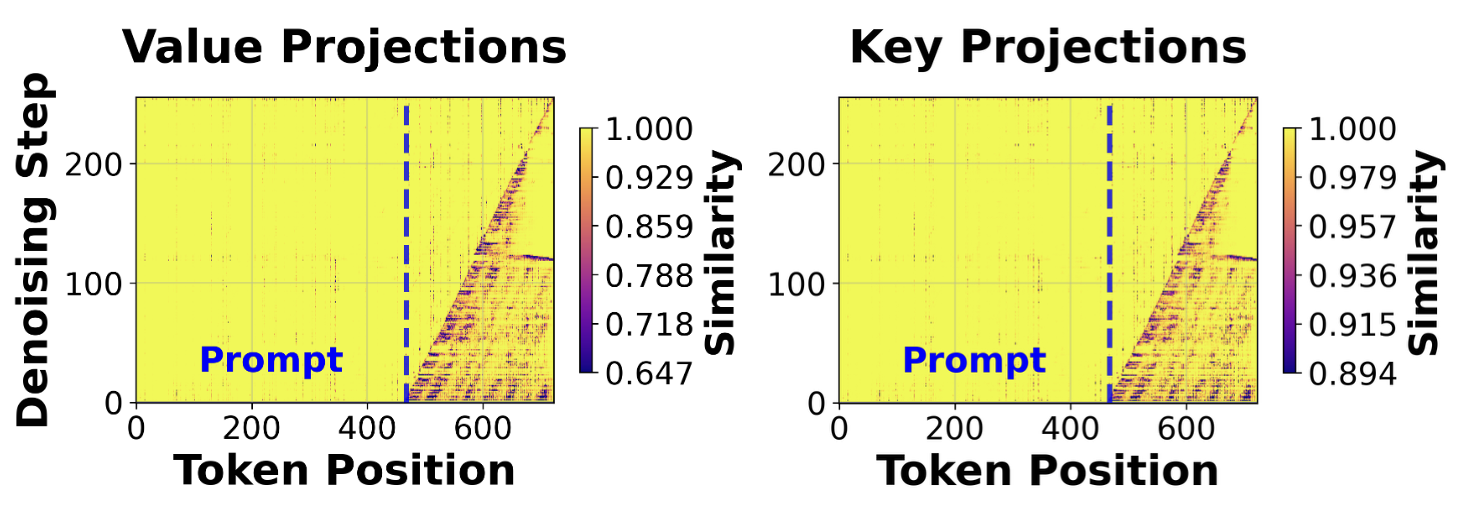
\includegraphics[width=1\linewidth]{sections/method/figures/kv_projections.png}
%     \caption{Rationale behind the proposed FreeCache: The variation of K and V projections of clean tokens is small throughout the subsequent diffusion steps. }
%     \label{fig:freecache_rationale}
% \end{figure}

\begin{table}[t!]
\caption{Latency and accuracy of the proposed FreeCache with different Diffusion Language Models. The proposed method achieves 4.42$\times$ and 6.32$\times$ speedup on Dream-7B-Instruct and LLaDA-8B-Instruct models.}
\label{tab:freecache_results}
\resizebox{\linewidth}{!}{\begin{tabular}{ccccc}
\toprule
\textbf{Models}                             & \textbf{Method}                & \textbf{GSM8K (8-shot) Accuracy (\%)} & \textbf{Raw Latency (s)} & \textbf{Speedup}       \\ \midrule
\multirow{2}{*}{Dream-7B-Instruct~\cite{dream2025}} & Baseline              & 79.68               & 48.05           & 1.0 $\times$  \\ \cmidrule{2-5} 
                                   & \textbf{FreeCache (This work)} & 77.40               & \textbf{10.87}           & \textbf{4.42}$\times$  \\ \midrule
\multirow{2}{*}{LLaDA-8B-Instruct~\cite{nie2025large}}          & Baseline              & 79.30               & 56.89           & 1.0 $\times$  \\ \cmidrule{2-5} 
                                   & \textbf{FreeCache (This work)} & 77.18               & \textbf{9.02}            & \textbf{6.32}$\times$ \\ \bottomrule
\end{tabular}}
\end{table}





\subsubsection{Guiding Diffusion with Lightweight Autoregressive Model}


% The beauty of diffusion model is the ability of producing tokens without relying on the iterative decoding process, whereas the inc
To address this token incoherence challenge~(Challenge \circled{2}) from Section~\ref{sec:incor}
and fully exploit the parallelism of diffusion process, we propose \texttt{Guided Diffusion}. 
% \begin{figure}[t!]
\vspace{-6pt}
\begin{figure}[H]
    \centering
    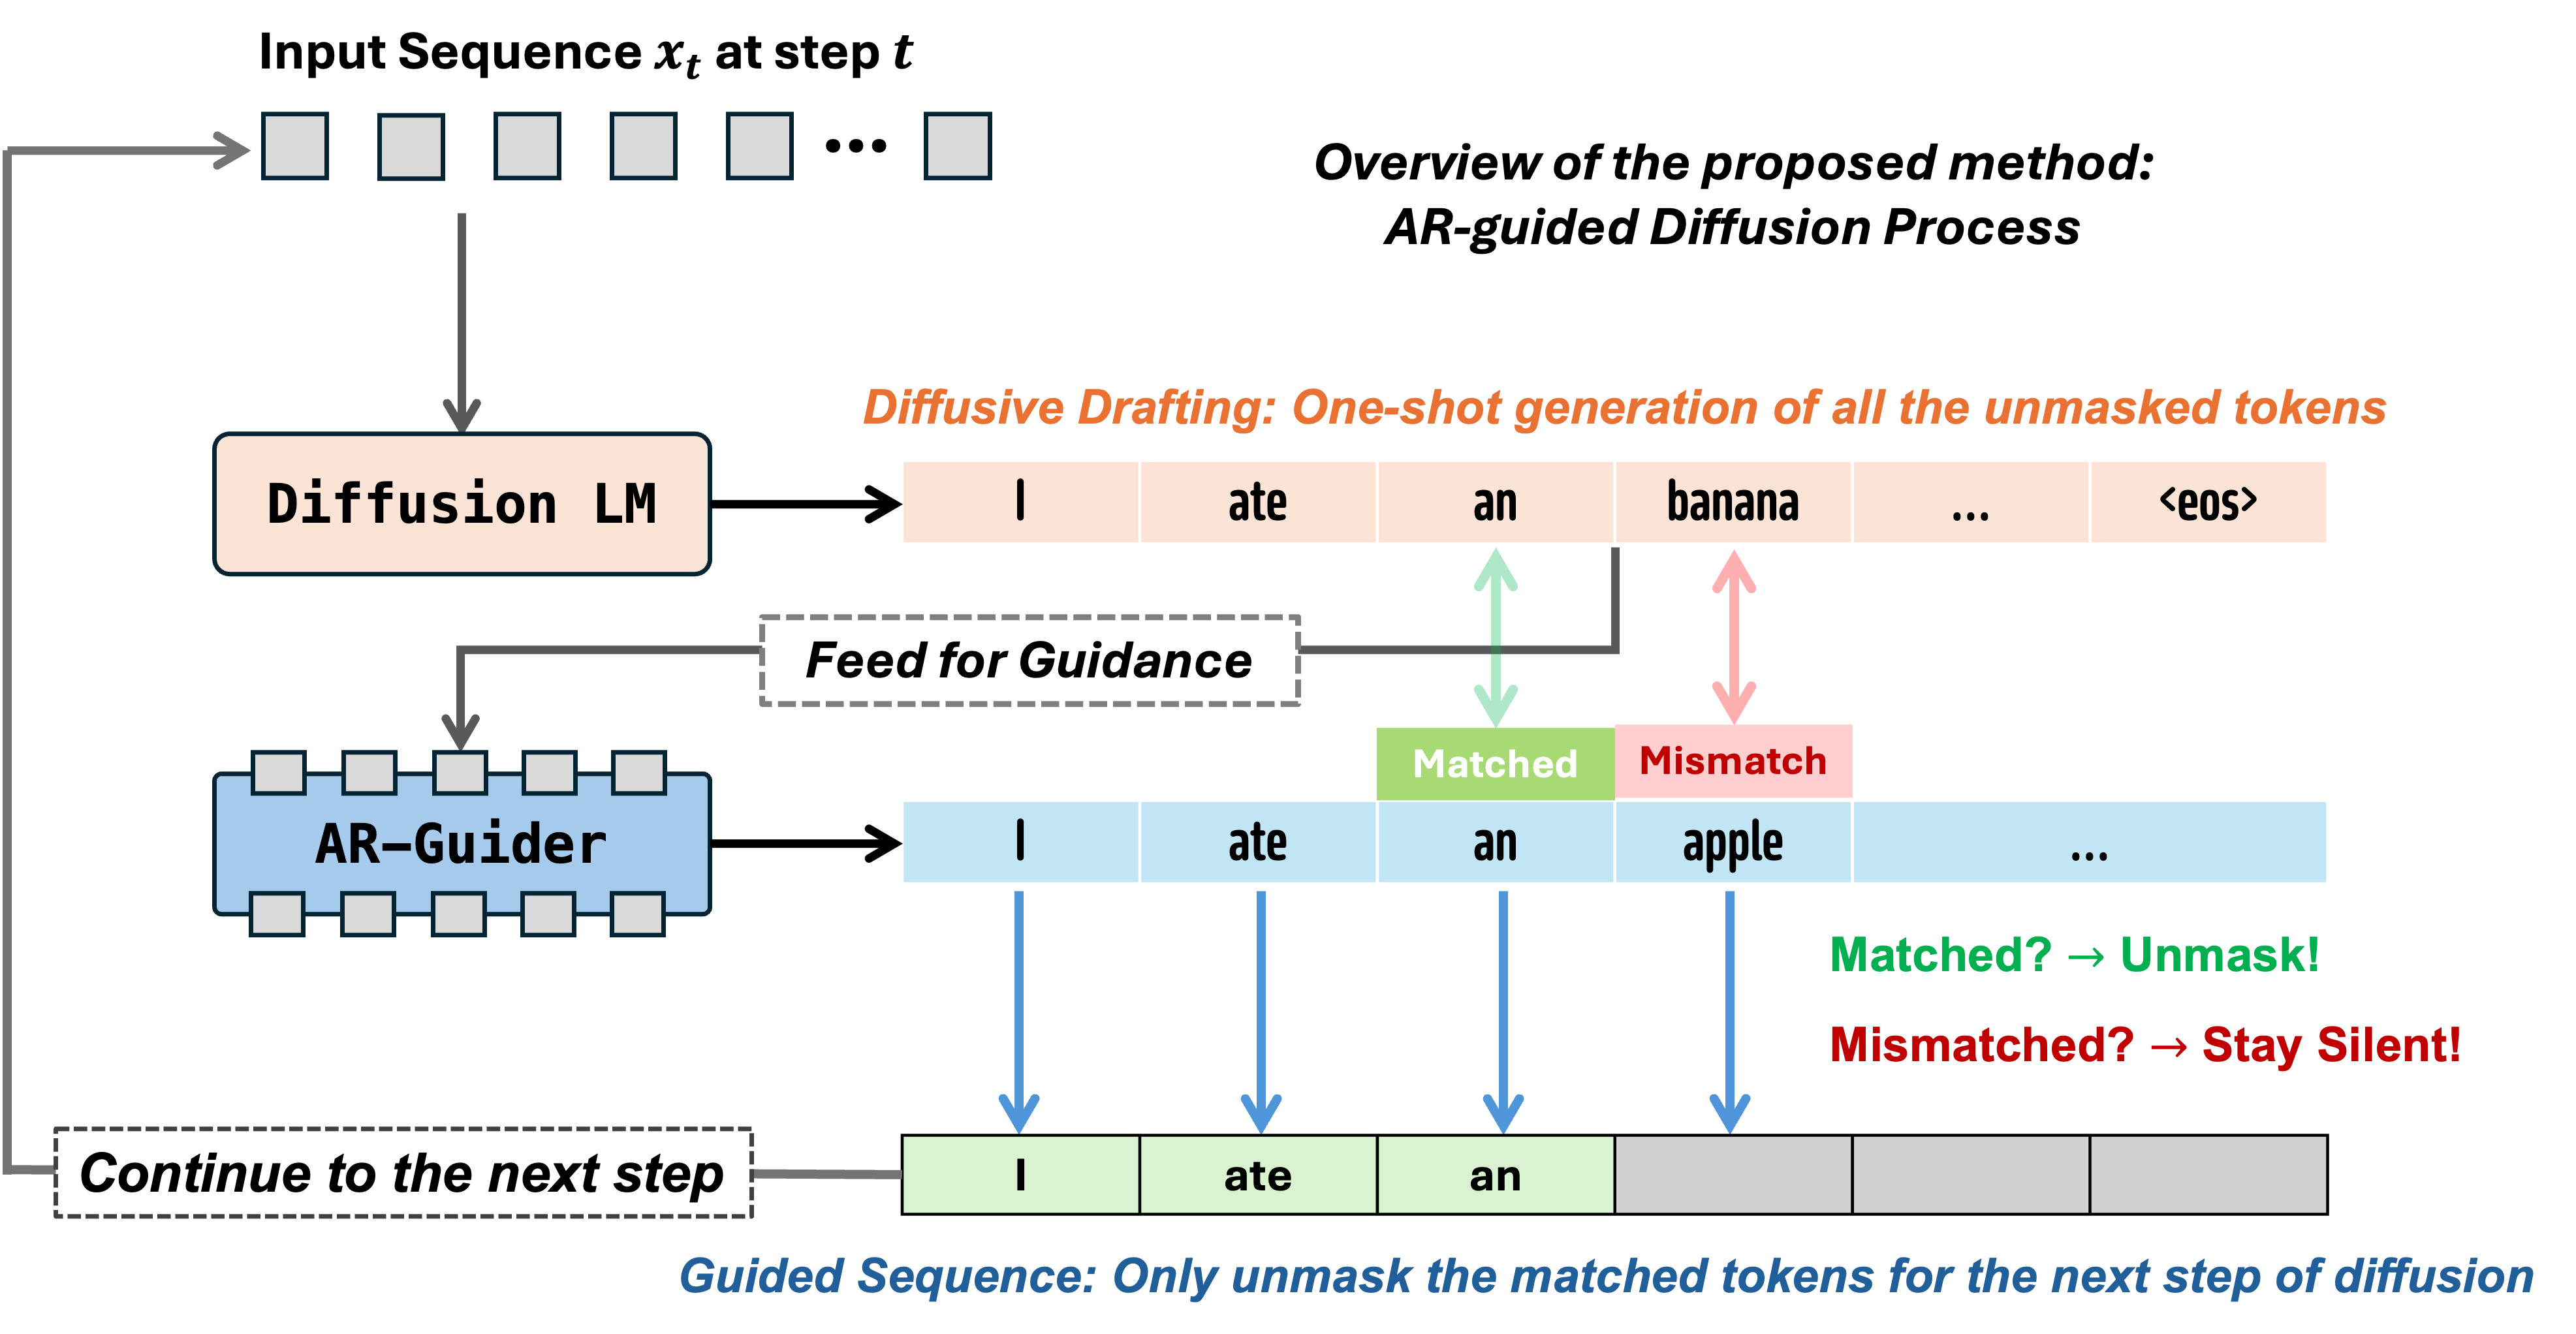
\includegraphics[width=\linewidth]{sections/method/figures/guided_diffusion.png}
    \caption{AR-guided Diffusion Model. The diffusion model performs a one-step diffusion process, followed by a one-time forward pass of the AR guider. The matched tokens are unmasked for the next step of diffusion.}
    \label{fig:guided_diffusion}
\end{figure}
\vspace{-6pt}

Specifically, we leverage the diffusion model as the ``drafter'' model by first unmasking \textbf{all} the tokens with one step. 
The masked tokens predicted by the diffusion model are only unmasked when they are consistent with the predictions from the autoregressive LM model, as shown in Figure~\ref{fig:guided_diffusion}. 
For the scenario when the matching ratio between the diffusion drafter and auto-regressive model is zero, the guided diffusion will only accept the one free tokens from the AR model output. 

This cross-model agreement serves as a lightweight coherence prior, enabling the model to safely unmask multiple tokens in parallel, without requiring any additional training or fine-tuning.

% In contrast to prior heuristic-based methods (e.g., confidence thresholds or top-$k$ logits), which often suffer from severe quality degradation when unmasking more than a few tokens per step, guided diffusion maintains fluency and correctness even under aggressive unmasking. This substantially reduces the number of denoising steps, often by a factor of 5× or more, without compromising output quality.

% We provide detailed comparisons in Section~\ref{sec:experiments}, \zhanqiu{TODO} showing that guided diffusion achieves significantly faster inference and stronger generation quality compared to baseline sampling strategies.


Guided diffusion performs iterative unmasking by coordinating predictions from a diffusion language model (DLM) and a frozen autoregressive model (ARM). At each denoising step, instead of relying on heuristic confidence thresholds, it uses agreement between the two models to decide how many tokens to safely unmask.

Formally, let \( x_T \in \mathbb{N}^L \) be the current sequence containing masked and unmasked tokens. The diffusion model \( f_\theta \) predicts logits over vocabulary tokens at all masked positions, from which we take the Top-1 predictions:
\[
t^{\text{DLM}} = \text{argmax}( \operatorname{Softmax}(f_\theta(x))).
\]
These proposed tokens are fed to the ARM \( g_\phi \), which produces a second set of logits:
\[
t^{\text{ARM}} = \text{argmax}( \operatorname{Softmax}(g_\phi(t^{\text{DLM}}))).
\]
Let \( M = [i_1, \dots, i_m] \subseteq \{1, \dots, L\} \) denote the current masked positions in \(x\). We compute the largest prefix length \(k\) such that
\[
t^{\text{DLM}}_{i_j} = t^{\text{ARM}}_{i_j} \quad \text{for all } j \le k.
\]
If \(k > 0\), we unmask positions \(i_1, \dots, i_k\) using the DLM proposals. If no agreement is found, we conservatively unmask only the first token \(i_1\). This process is repeated until all tokens are unmasked.

This decoding strategy allows the model to adaptively control the amount of parallel unmasking based on model confidence and alignment, enabling efficient generation without compromising output quality.
We present the details of the proposed method in Algorithm~\ref{alg:guided_diffusion}.

We would like to highlight that the proposed \texttt{Guided Diffusion} properly combines the advantages of \textbf{both} diffusion model and auto-regressive model. 
For each guiding step, \textbf{both} one-time diffusion process from the drafter and the one-time forward pass of the auto-regressive model are fast, while the guidance from the auto-regressive model facilitates the coherence of the diffused output tokens with improved semantical logic. 

\textbf{Guided Diffusion vs. Speculative Decoding.} 
Unlike speculative decoding, \texttt{Guided Diffusion} does not require token-wise correction from the auto-regressive model. In other words, the proposed method produces output sequence \textbf{without} introducing the repetitive correction process, which guarantees the latency benefits obtained from the fast diffusion process. 
Speculative decoding uses a small AR model for autoregressive drafting, followed by the big model correction. On the contrary, the proposed guided diffusion flips the paradigm by maximizing the drafting efficiency of the big diffusion model. To that end, the reasoning power of the diffusion model is fully preserved, while the AR guider model simply ensures the causality of the output. 


% In the meantime, Guided Diffusion can be smoothly transformed into ``Guided Correction''. The correction step can be directly applied after selecting the optimal tokens for unmasking. 
% In particular, when a stronger or domain-specific auto-regressive model is available, we can optionally apply a correction step that overwrites the diffusion draft with the accurate output from the expert auto-regressive model, as presented in Algorithm~\ref{alg:guided_diffusion_corrected}. We presented the detailed results 

%The original algorithm relies entirely on the diffusion model’s generation, but when a stronger or domain-specific ARM is available, we can optionally apply a correction step that overwrites the diffusion model’s proposal using the ARM’s prediction to improve accuracy, as shown in Algorithm~\ref{alg:guided_diffusion_corrected}.





% GUided only
% \begin{algorithm}[H]
%   \caption{Guided Diffusion}
%   \label{alg:guided_diffusion}
%   \begin{algorithmic}[1]
%     \REQUIRE initial masked sequence \(x\), diffusion model \(f_\theta\), AR model \(g_\phi\)
%     \ENSURE fully unmasked sequence \(x\)
%     \WHILE{\(\exists i:\;x[i]=\mathrm{mask}\)}
%       \STATE \(\mathrm{dlm\_logits}\gets\operatorname{softmax}\bigl(f_\theta(x)\bigr)\)
%       \STATE \(\mathrm{dlm\_tokens}\gets\arg\max\,\mathrm{dlm\_logits}\)
%       \STATE \(\mathrm{ar\_logits}\gets\operatorname{softmax}\bigl(g_\phi(\mathrm{dlm\_tokens})\bigr)\)
%       \STATE \(\mathrm{ar\_tokens}\gets\arg\max\,\mathrm{ar\_logits}\)
%       \STATE let $M$ be the masked indices of \(x\)
%       \STATE 
%         \(k \gets \max\{\,j : \mathrm{dlm\_tokens}_{i_\ell}
%         = \mathrm{ar\_tokens}_{i_\ell}\ \forall\ell\le j\}\)
%       \IF{\(k>0\)}
%         \STATE unmask \(i_1,\dots,i_k\) in \(x\) with \(\mathrm{dlm\_tokens}_{i_1\ldots i_k}\)
%       \ELSE
%         \STATE unmask \(i_1\) in \(x\) with \(\mathrm{dlm\_tokens}_{i_1}\)
%       \ENDIF
%     \ENDWHILE
%   \end{algorithmic}
% \end{algorithm}

% \begin{figure}[h!]
%   \centering
%   %----------- Guided Diffusion (Left) -----------%
%   \begin{minipage}[t]{0.49\columnwidth}
%     \begin{algorithm}[H]
%       \caption{Guided Diffusion (AR-Assisted)}
%       \label{alg:guided_diffusion}
%       \begin{algorithmic}[1]
%         \REQUIRE masked seq.\ \(x\), DLM \(f_\theta\), AR \(g_\phi\)
%         \ENSURE fully unmasked \(x\)
%         \WHILE{\(\exists i:\,x[i] = \text{mask}\)}
%           \STATE \( \text{log}_d \gets \operatorname{softmax}(f_\theta(x)) \)
%           \STATE \( \text{tok}_d \gets \arg\max\, \text{log}_d \)
%           \STATE \( \text{log}_a \gets \operatorname{softmax}(g_\phi(\text{tok}_d)) \)
%           \STATE \( \text{tok}_a \gets \arg\max\, \text{log}_a \)
%           \STATE let \( M = [i_1, \dots, i_m] \) be masked indices
%           \STATE \( k \gets \max\{ j : \text{tok}_d[i_\ell] = \text{tok}_a[i_\ell],\, \forall \ell \le j \} \)
%           \IF{\(k > 0\)}
%             \STATE unmask \(i_1{:}i_k\) with \(\text{tok}_d[i_1{:}i_k]\)
%           \ELSE
%             \STATE unmask \(i_1\) with \(\text{tok}_d[i_1]\)
%           \ENDIF
%         \ENDWHILE
%       \end{algorithmic}
%     \end{algorithm}
%   \end{minipage}%
%   \hspace{2pt}
%   %-------- Guided Diffusion + Correction (Right) --------%
%   \begin{minipage}[t]{0.49\columnwidth}
%     \begin{algorithm}[H]
%       \caption{Guided Diffusion with Correction}
%       \label{alg:guided_diffusion_corrected}
%       \begin{algorithmic}[1]
%         \REQUIRE masked seq.\ \(x\), DLM \(f_\theta\), AR \(g_\phi\)
%         \ENSURE fully unmasked \(x\)
%         \WHILE{\(\exists i:\,x[i] = \text{mask}\)}
%           \STATE \( \text{log}_d \gets \operatorname{softmax}(f_\theta(x)) \)
%           \STATE \( \text{tok}_d \gets \arg\max\, \text{log}_d \)
%           \STATE \( \text{log}_a \gets \operatorname{softmax}(g_\phi(\text{tok}_d)) \)
%           \STATE \( \text{tok}_a \gets \arg\max\, \text{log}_a \)
%           \STATE let \( M = [i_1, \dots, i_m] \) be masked indices
%           \STATE \( k \gets \max\{ j : \text{tok}_d[i_\ell] = \text{tok}_a[i_\ell],\, \forall \ell \le j \} \)
%           \IF{\(k > 0\)}
%             \STATE unmask \(i_1{:}i_k\) with \(\text{tok}_d[i_1{:}i_k]\)
%             \STATE unmask \(i_{k+1}\) with \(\text{tok}_a[i_{k+1}]\)
%           \ELSE
%             \STATE unmask \(i_1\) with \(\text{tok}_d[i_1]\)
%           \ENDIF
%         \ENDWHILE
%       \end{algorithmic}
%     \end{algorithm}
%   \end{minipage}
%   % \caption{Left: AR-assisted guided diffusion. Right: with correction—also fills one token using AR beyond matched region.}
% \end{figure}




% \begin{figure}[h!]
%   \centering
%   %----------- Guided Diffusion (Left) -----------%
%   \begin{minipage}[t]{0.49\columnwidth}
%     \begin{algorithm}[H]
%       \caption{Guided Diffusion}
%       \label{alg:guided_diffusion}
%       \begin{algorithmic}[1]
%         \REQUIRE masked seq.\ \(x\), DLM \(f_\theta\), AR \(g_\phi\)
%         \ENSURE fully unmasked \(x\)
%         \WHILE{\(\exists i:\,x[i] = \text{mask}\)}
%           \STATE \( \text{logits}_{DLM} \gets \operatorname{softmax}(f_\theta(x)) \)
%           \STATE \( \text{tok}_{DLM} \gets \arg\max\, \text{logits}_{DLM} \)
%           \STATE \( \text{logits}_{AR} \gets \operatorname{softmax}(g_\phi(\text{tok}_{DLM})) \)
%           \STATE \( \text{tok}_{AR} \gets \arg\max\, \text{logits}_{AR} \)
%           \STATE let \( M = [i_1, \dots, i_m] \) be masked indices
%           \STATE \( k \gets \max\{ j : \text{tok}_{DLM}[i_\ell] = \text{tok}_{AR}[i_\ell],\, \forall \ell \le j \} \)
%           \IF{\(k > 0\)}
%             \STATE unmask \(i_1{:}i_k\) with \(\text{tok}_{DLM}[i_1{:}i_k]\)
%           \ELSE
%             \STATE unmask \(i_1\) with \(\text{tok}_{DLM}[i_1]\)
%           \ENDIF
%         \ENDWHILE
%       \end{algorithmic}
%     \end{algorithm}
%   \end{minipage}%
%   \hspace{2pt}
%   %-------- Guided Diffusion + Correction (Right) --------%
%   \begin{minipage}[t]{0.49\columnwidth}
%     \begin{algorithm}[H]
%       \caption{Guided Diffusion with Correction}
%       \label{alg:guided_diffusion_corrected}
%       \begin{algorithmic}[1]
%         \REQUIRE masked seq.\ \(x\), DLM \(f_\theta\), AR \(g_\phi\)
%         \ENSURE fully unmasked \(x\)
%         \WHILE{\(\exists i:\,x[i] = \text{mask}\)}
%           \STATE \( \text{logits}_{DLM} \gets \operatorname{softmax}(f_\theta(x)) \)
%           \STATE \( \text{tok}_{DLM} \gets \arg\max\, \text{logits}_{DLM} \)
%           \STATE \( \text{logits}_{AR} \gets \operatorname{softmax}(g_\phi(\text{tok}_{DLM})) \)
%           \STATE \( \text{tok}_{AR} \gets \arg\max\, \text{logits}_{AR} \)
%           \STATE let \( M = [i_1, \dots, i_m] \) be masked indices
%           \STATE \( k \gets \max\{ j : \text{tok}_{DLM}[i_\ell] = \text{tok}_{AR}[i_\ell],\, \forall \ell \le j \} \)
%           \IF{\(k > 0\)}
%             \STATE unmask \(i_1{:}i_k\) with \(\text{tok}_{DLM}[i_1{:}i_k]\)
%             \STATE unmask \(i_{k+1}\) with \(\text{tok}_{AR}[i_{k+1}]\)
%           \ELSE
%             \STATE unmask \(i_1\) with \(\text{tok}_{DLM}[i_1]\)
%           \ENDIF
%         \ENDWHILE
%       \end{algorithmic}
%     \end{algorithm}
%   \end{minipage}
%   % \caption{Left: AR-assisted guided diffusion. Right: with correction—also fills one token using AR beyond matched region.}
% \end{figure}



% \begin{figure}[h!]
%   \centering
%   %----------- Guided Diffusion (Left) -----------%
%   \begin{minipage}[t]{0.49\columnwidth}
%     \begin{algorithm}[H]
%       \caption{Guided Diffusion (AR-Assisted)}
%       \label{alg:guided_diffusion}
%       \begin{algorithmic}[1]
%         \REQUIRE masked seq.\ \(x\), DLM \(f_\theta\), AR \(g_\phi\)
%         \ENSURE fully unmasked \(x\)
%         \WHILE{\(\exists i:\,x[i] = \text{mask}\)}
%           \STATE \( \text{logits}_{\text{DLM}} \gets \operatorname{softmax}(f_\theta(x)) \)
%           \STATE \( \text{tok}_{\text{DLM}} \gets \arg\max\, \text{logits}_{\text{DLM}} \)
%           \STATE \( \text{logits}_{AR} \gets \operatorname{softmax}(g_\phi(\text{tok}_{\text{DLM}})) \)
%           \STATE \( \text{tok}_{\text{\text{AR}}} \gets \arg\max\, \text{logits}_{\text{AR}} \)
%           \STATE let \( M = [i_1, \dots, i_m] \) be masked indices
%           \STATE \( k \leftarrow \text{size}(\{\text{tok}_{\text{DLM}} = \text{tok}_{\text{AR}}\}) \)
%           \IF{\(k > 0\)}
%             \STATE Unmask \(i_1{:}i_k\) with \(\text{tok}_{\text{DLM}}[i_1{:}i_k]\)
%           \ELSE
%             \STATE Unmask \(i_1\) with \(\text{tok}_{\text{DLM}}[i_1]\)
%           \ENDIF
%         \ENDWHILE
%       \end{algorithmic}
%     \end{algorithm}
%   \end{minipage}%
%   \hspace{2pt}
%   %-------- Guided Diffusion + Correction (Right) --------%
%   \begin{minipage}[t]{0.49\columnwidth}
%     \begin{algorithm}[H]
%       \caption{Guided Diffusion with Correction}
%       \label{alg:guided_diffusion_corrected}
%       \begin{algorithmic}[1]
%         \REQUIRE masked seq.\ \(x\), DLM \(f_\theta\), AR \(g_\phi\)
%         \ENSURE fully unmasked \(x\)
%         \WHILE{\(\exists i:\,x[i] = \text{mask}\)}
%           \STATE \( \text{logits}_{\text{DLM}} \gets \operatorname{softmax}(f_\theta(x)) \)
%           \STATE \( \text{tok}_{\text{DLM}} \gets \arg\max\, \text{logits}_{\text{DLM}} \)
%           \STATE \( \text{logits}_{\text{AR}} \gets \operatorname{softmax}(g_\phi(\text{tok}_{\text{DLM}})) \)
%           \STATE \( \text{tok}_{\text{AR}} \gets \arg\max\, \text{logits}_{\text{AR}} \)
%           \STATE let \( M = [i_1, \dots, i_m] \) be masked indices
%           \STATE \( k \leftarrow \text{size}(\{\text{tok}_{\text{DLM}} = \text{tok}_{\text{AR}}\}) \)
%           \STATE Unmask \(i_1{:}i_k\) with \(\text{tok}_{\text{DLM}}[i_1{:}i_k]\)
%           \STATE Correct \(i_{k+1}\) with \(\text{tok}_{\text{AR}}[i_{k+1}]\)
%         \ENDWHILE
%       \end{algorithmic}
%     \end{algorithm}
%   \end{minipage}
%   % \caption{Left: AR-assisted guided diffusion. Right: with correction—also fills one token using AR beyond matched region.}
% \end{figure}



% \begin{figure}[h!]
%   \centering
%   \begin{minipage}[t]{\columnwidth} % Changed width to full column
%     \begin{algorithm}[H]
%       \caption{Guided Diffusion (AR-Assisted)}
%       \label{alg:guided_diffusion}
%       \begin{algorithmic}[1]
%         \REQUIRE masked seq.\ \(x\), DLM \(f_\theta\), AR \(g_\phi\)
%         \ENSURE fully unmasked \(x\)
%         \WHILE{\(\exists i:\,x[i] = \text{mask}\)}
%           \STATE \( \text{logits}_{\text{DLM}} \gets \operatorname{softmax}(f_\theta(x)) \)
%           \STATE \( \text{tok}_{\text{DLM}} \gets \arg\max\, \text{logits}_{\text{DLM}} \)
%           \STATE \( \text{logits}_{\text{AR}} \gets \operatorname{softmax}(g_\phi(\text{tok}_{\text{DLM}})) \)
%           \STATE \( \text{tok}_{\text{\text{AR}}} \gets \arg\max\, \text{logits}_{\text{AR}} \)
%           \STATE let \( M = [i_1, \dots, i_m] \) be masked indices
%           \STATE \( k \leftarrow \text{size}(\{\text{tok}_{\text{DLM}} = \text{tok}_{\text{AR}}\}) \)
%           \IF{\(k > 0\)}
%             \STATE Unmask \(i_1{:}i_k\) with \(\text{tok}_{\text{DLM}}[i_1{:}i_k]\)
%           \ELSE
%             \STATE Unmask \(i_1\) with \(\text{tok}_{\text{DLM}}[i_1]\)
%           \ENDIF
%         \ENDWHILE
%       \end{algorithmic}
%     \end{algorithm}
%   \end{minipage}
% \end{figure}




\begin{figure}[h!]
  \centering
  \begin{minipage}[t]{\columnwidth}
    \begin{algorithm}[H]
      \caption{Guided Diffusion}
      \label{alg:guided_diffusion}
      \KwIn{masked sequence $x$, DLM $f_\theta$, AR $g_\phi$}
      \KwOut{fully unmasked $x$}

      \While{$\exists i:\,x[i] = \text{mask}$ \tcp*[f]{loop until all unmasked~}}{
        $\text{logits}_{\text{DLM}} \gets \operatorname{softmax}(f_\theta(x))$ \tcp*[f]{DLM predicts masked tokens}\\
        $\text{tok}_{\text{DLM}} \gets \arg\max \text{logits}_{\text{DLM}}$ \tcp*[f]{DLM predictions}\\
        $\text{logits}_{\text{AR}} \gets \operatorname{softmax}(g_\phi(\text{tok}_{\text{DLM}}))$ \tcp*[f]{AR processes DLM output}\\
        $\text{tok}_{\text{AR}} \gets \arg\max \text{logits}_{\text{AR}}$ \tcp*[f]{AR predictions}\\
        Let $M = [i_1,\dots,i_m]$ be masked indices \tcp*[f]{remaining mask positions}\\
        $k \leftarrow \text{size}(\{\text{tok}_{\text{DLM}} = \text{tok}_{\text{AR}}\})$ \tcp*[f]{find matches}\\

        \eIf{$k > 0$ \tcp*[f]{models agree~}}{
          Unmask $i_1{:}i_k$ with $\text{tok}_{\text{DLM}}[i_1{:}i_k]$ \tcp*[f]{accept matching run}
        }{
          Unmask $i_1$ with $\text{tok}_{\text{DLM}}[i_1]$ \tcp*[f]{fallback:~accept first}
        }
      }
    \end{algorithm}
  \end{minipage}
\end{figure}
